\chapter{绪论}\label{chp:introduction}

\section{研究背景及意义}\label{sec:background_and_significance}

近年以来，以大语言模型（Large Language Models, LLMs）\cite{zhao2026survey,minaee2025large,min2023recent}为代表的生成式人工智能技术取得了突破性进展。得益于海量语料训练与大规模参数建模能力，LLM在自然语言理解与生成任务中展现出了卓越的性能，在机器翻译、智能问答、文本摘要、代码生成以及对话系统等多个领域取得了广泛应用。以GPT\cite{radford2018improving,radford2019language,brown2020language,achiam2023gpt}、LLaMA\cite{touvron2023llama,touvron2023llama2,grattafiori2024llama}、Qwen\cite{bai2023qwen,yang2025qwen3}等模型为代表的大语言模型已经逐渐成为智能信息处理系统的重要基础设施，并被广泛集成于搜索引擎、智能助手、教育辅助、医疗咨询以及知识管理等实际应用场景中。

尽管大语言模型在生成能力和语言理解能力方面取得了显著进展，但其在生成过程中仍然存在一个重要问题，即“幻觉”（Hallucination）\cite{huang2025survey,ji2023survey,geng2024survey}。所谓幻觉，是指模型在生成文本时产生与事实不符、逻辑错误或缺乏依据的内容。例如，模型可能生成不存在的参考文献、错误的事实描述、虚构的实体关系，甚至给出看似合理但实际上并不正确的推理结论。由于大语言模型本质上是基于概率分布采样进行文本生成的，其生成过程并不直接依赖真实世界知识验证，因此在缺乏可靠约束的情况下容易产生此类错误信息。

幻觉问题在实际应用中可能带来严重影响。在智能问答系统中，幻觉可能导致错误信息的传播；在医疗、法律、自动驾驶等高风险领域，错误的生成内容甚至可能造成决策风险；在知识检索与信息整合任务中，虚构事实或错误引用也会严重降低系统的可信度。因此，如图~\ref{fig:hallucination_detection_types}左半部分所示，幻觉检测（Hallucination Detection）\cite{luo2024hallucination}这一研究领域应运而生，旨在有效识别和检测大语言模型生成过程中的幻觉内容，并已经成为当前大模型安全性与可靠性研究中的关键问题之一。近年来，研究者提出了多种幻觉检测与评估方法，试图从不同角度识别模型生成结果的真实性与可靠性，从而提高大语言模型在实际应用中的可信度。

\begin{figure}[htbp]
    \centering
    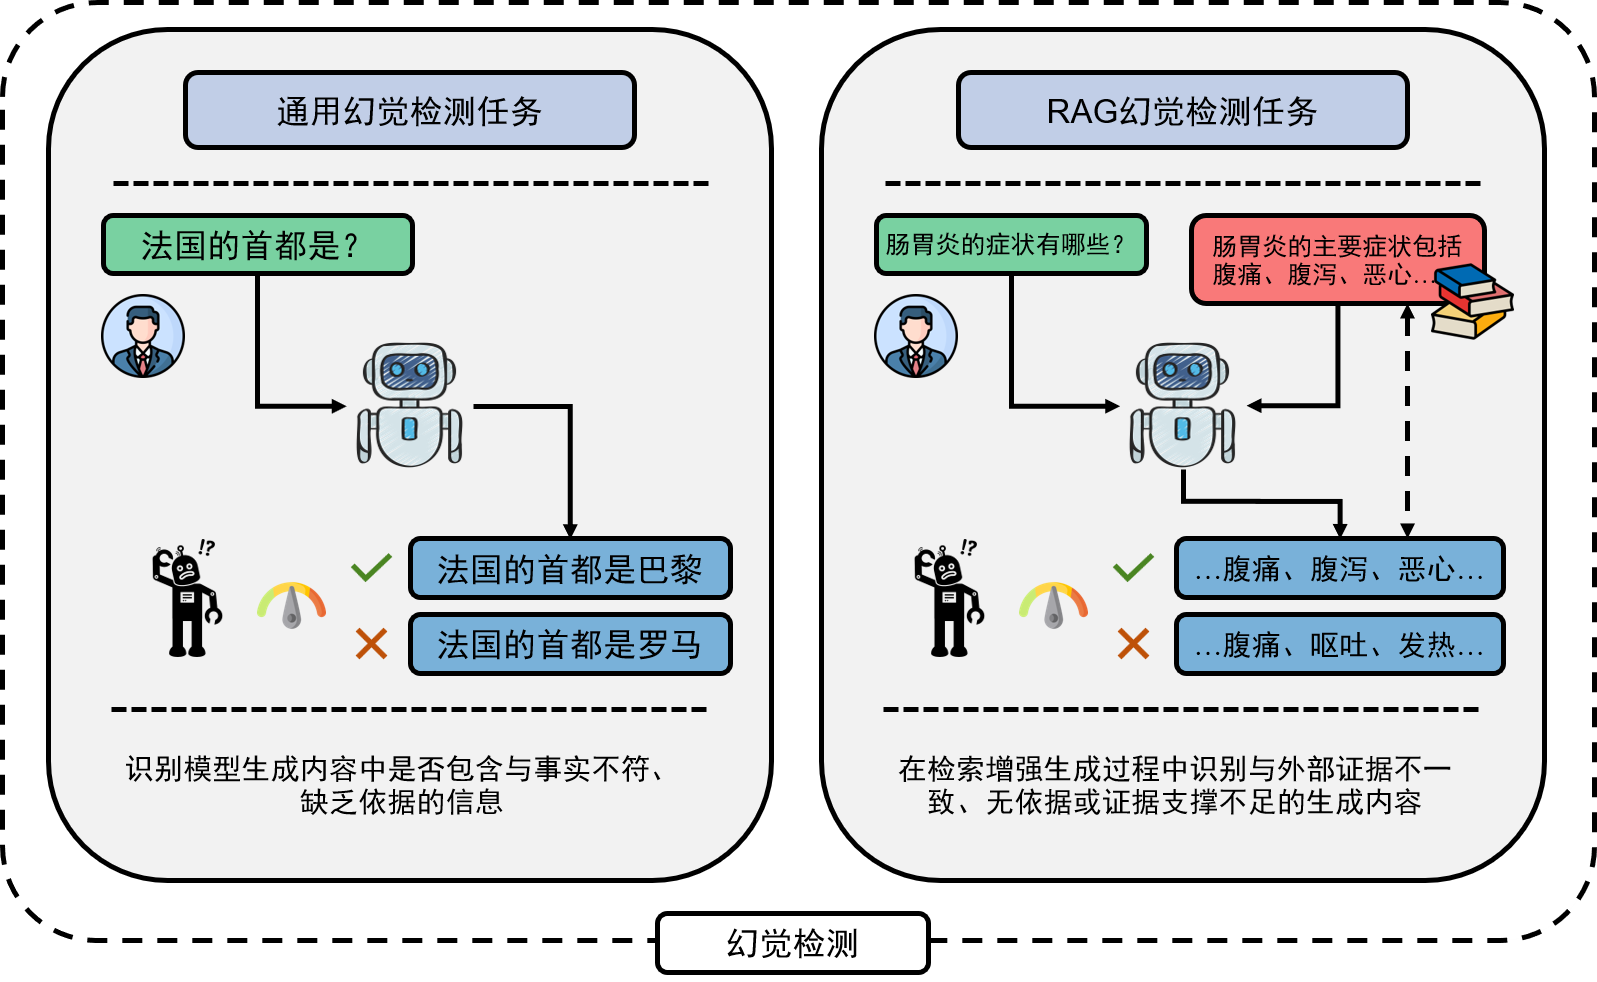
\includegraphics[width=\textwidth]{figures/content/幻觉检测类型.png}
    \caption{本文讨论的两类幻觉检测任务示例图}\label{fig:hallucination_detection_types}
\end{figure}

为了缓解大语言模型中由于知识不完整或事实不准确所带来的幻觉问题，研究者提出了检索增强生成（Retrieval-Augmented Generation, RAG）\cite{gao2024retrieval,huang2024survey,wu2025retrieval}框架。RAG通过在输入端或生成过程中引入外部知识检索机制，使模型能够结合实时或高质量的知识库信息进行文本生成，从而大幅提高生成内容的事实准确性和可解释性。然而，在实际应用中，受限于大模型本质的输出概率采样机制，RAG系统仍然难以完全避免幻觉现象。当模型内部知识与检索得到的外部知识之间存在冲突时，即便提供有给定的检索知识上下文，模型也可能忽略检索到的证据，依然依据自身参数化知识生成内容，从而产生与检索知识不一致的结果。因此，即便在引入外部知识的情况下，RAG系统仍可能出现幻觉问题，这一新的幻觉形式通常被称为RAG幻觉或检索增强生成幻觉（RAG Hallucination），如图~\ref{fig:hallucination_detection_types}右半部分所示。

一类简单的幻觉检测方法是依赖于生成不确定性、自一致性分析的黑盒方法。此类方法简单易用，具有较好的模型通用性，但往往只能利用有限的输出信息，对模型内部表征的利用较为有限；并因常需要采样多次输出，通常有较高的计算资源开销。因此，在对时效、算力或性能要求较高场景下的检测能力仍然存在一定局限。事实上，大语言模型在推理过程中会产生大量隐藏状态（hidden state），这些内部表征在不同层次上反映了模型对输入语义、上下文信息以及知识结构的理解。如何有效挖掘并利用这些内部表征信息，为幻觉检测提供更加稳定和可靠的判别依据，成为当前值得深入研究的重要方向\cite{skean2025layer,laptev2025analyze}。此外，在检索增强生成场景下，通过在模型内部表征空间分析内部参数化知识与外部检索知识之间的关系，也有望更准确地检测生成内容与检索知识之间的潜在冲突。

基于上述背景，研究基于内部表征的幻觉检测方法，对于提升生成式人工智能系统的安全性与可信度具有重要意义。一方面，通过充分分析模型内部表征结构，可以在不依赖大量标注数据的情况下实现更加通用的幻觉检测；另一方面，在RAG场景下，通过在内部表征空间对模型参数化知识与外部检索知识之间进行冲突消解，也能够进一步提高对输出检测结果的真实性与可靠性。因此，探索基于内部表征的大语言模型幻觉检测方法，对于推动大语言模型在复杂实际场景中的安全应用具有重要研究价值和应用意义。

\section{研究现状及挑战}\label{sec:current_status_and_challenges}

\subsection{通用幻觉检测}\label{subsec:hallucination_detection}

大语言模型幻觉检测（Hallucination Detection）\cite{luo2024hallucination}通常指识别模型生成内容中是否包含与事实不符、缺乏依据或与上下文知识不一致的信息。与传统自然语言处理任务不同，幻觉检测并不直接关注文本生成质量本身，而是侧重于判断生成内容的真实性与可靠性。随着大语言模型在问答系统、知识检索和对话系统中的广泛应用，如何自动识别生成文本中的潜在幻觉，已经成为当前大模型安全性与可信性研究中的重要问题。现有研究通常从不同角度对幻觉检测问题进行建模，主要可以分为两大类方法：一类是基于生成概率、不确定性或自一致性的检测方法，其特点是无需获取模型内部表征，因此亦称“黑盒方法”；另一类为基于内部隐藏状态、激活表示或探针的检测方法，其特点是需要访问模型内部表征信息以进行检测，因此亦称“白盒方法”。

\subsubsection{基于生成概率、不确定性或自一致性的幻觉检测（黑盒方法）}

在黑盒方法的设定下，模型被假设为不可观测内部参数的封闭系统，仅能通过输入输出接口进行交互。其基本思想是通过分析模型生成过程中的概率特征、生成稳定性或多次生成结果之间的一致性，判断当前输出是否存在潜在的不可靠信息。此类方法的理论基础源于“一致性假设”，即——因模型对参数化知识的概率拟合特性，同一幻觉内容的复现在多次随机采样条件下呈现显著的随机性特征。由于此类方法无需访问模型内部参数或隐藏状态，因此简单易用，具有较好的模型通用性，并且能够方便地应用于不同类型的大语言模型。然而，这类方法往往只能利用有限的输出信息，对模型内部知识表示的利用较为有限；并因常需要采样多次输出，通常有较高的计算资源开销。因此，在对时效、算力或性能要求较高场景下的检测能力仍然存在一定局限。

黑盒方法早期的一些工作采用较为简单的输出一致性度量作为幻觉检测信号。例如，Lexical Similarity类方法通过比较同一问题在多次采样生成的答案之间的词汇相似度（如Rouge-L\cite{lin2004rouge}等指标）来评估生成稳定性。如果多个输出之间在表述上存在较大差异，则可能意味着模型在生成过程中缺乏稳定的知识依据，从而具有较高的幻觉风险。尽管此类方法实现简单，但它们为后续基于一致性假设的检测方法奠定了基础，在许多后续文章\cite{manakul2023selfcheckgpt}中被作为比较基线。随后，方法SelfCheckGPT\cite{manakul2023selfcheckgpt}利用相同或额外的黑盒大语言模型对被测大语言模型的多个输出计算幻觉风险。具体地，SelfCheckGPT通过构造形如“<片段 A>是否支持<回复 1>”的问题，对来自不同采样结果中的片段与回复进行交叉验证，并统计回答“支持”的比例作为幻觉风险指标。若不同生成结果之间缺乏相互支持关系，则说明模型生成内容的一致性较弱，从而更可能包含幻觉信息。在此基础上，一些研究尝试利用概率结构或内部统计量对生成不确定性进行建模。例如，方法LLM-Check\cite{sriramanan2024llm}利用大模型内部中间层的token级别输出，并结合注意力矩阵进行特征值分解，通过计算矩阵的对数行列式作为幻觉指标。当该指标较高时，说明各批次输出或各token之间的相关性较弱，模型不确定度较高，从而更容易产生幻觉。尽管LLM-Check在计算过程中使用了模型的中间表示，但其特征提取过程可以在任意可访问内部状态的替代模型上完成，因此在实际应用中仍可视为一种黑盒检测策略。另一类方法进一步从语义层面刻画多次生成之间的一致性。例如，方法\citen{abdaljalil2025scalable}通过对同一问题的多个生成结果提取语义嵌入向量，计算各输出之间的余弦相似度，并利用层次聚类将其划分为多个语义簇。在此基础上，研究者提出以“语义熵”（semantic entropy）作为衡量生成稳定性的指标：当输出被划分为多个语义差异较大的簇时，说明模型对该问题缺乏稳定的知识表达，从而具有更高的幻觉风险。值得注意的是，该方法中的嵌入向量可以通过外部编码器获得，因此无需访问被测模型的内部表示。除了直接进行检测之外，还有一些工作尝试通过利用多次生成结果来缓解或减少幻觉现象。例如，方法Copy-Paste\cite{long2025copy}通过提示模型优先从给定上下文中复制相关信息来生成回答，从而得到质量更高、幻觉更少的响应。随后，这些高质量生成结果被用于对模型进行后训练（post-training），以进一步降低模型在开放域问答中的幻觉概率。尽管该方法的主要目标在于缓解幻觉问题，但其核心思想同样依赖于对模型生成一致性的分析，因此与黑盒检测方法在思想上具有一定关联。

除基于生成概率、不确定性或自一致性的幻觉检测方法之外，还存在一类简单直接的黑盒方法，即基于提示词的方法。此类方法通过提示工程（Prompt Engineering）设计特定指令或问题链引导大语言模型自我验证其生成内容的可靠性，其核心假设为：模型具备内生的事实性反思能力，可通过提示激发其对潜在矛盾的主动检测。例如，可以通过引导模型自主输出其对自身生成内容的不确定度等多种方式来检测幻觉。文献\citen{lin2022teaching}提出通过微调GPT-3模型使其直接生成自然语言形式的置信度表达（如“90\%置信度”或“高置信度”），而非依赖传统模型对数概率。 然而，此类方法极其依赖自我检查的框架流程设计和提示词设计的精细度，并且很大程度上受到模型自身理解和推理能力的制约；此外因需要多次多种提示词输入输出，计算开销显著高于常规推理。

\subsubsection{基于内部隐藏状态、激活表示或探针的幻觉检测（白盒方法）}

白盒方法通常假设大语言模型内部的所有中间参数在推理过程中均可见，如模型对所有token的输出概率分布，模型中间某层的注意力参数等等。此类方法的理论基础源于“不确定性假设”，即——类似人类说谎时一般，模型对生成幻觉内容的确定度较低，这种不确定性能够在模型内部参数中隐式表征出来。大语言模型在生成过程中会产生丰富的隐藏状态表示，这些内部表征在不同层次上反映了模型对语义结构、上下文信息以及知识关联的理解。通过分析这些内部表示的分布特性或结构特征，可以为幻觉检测提供更加细粒度的判别依据。与黑盒方法相比，这类方法通常能够更充分地利用模型内部信息，因此在检测能力方面具有一定优势，是当前学术界研究较为活跃的方向；同时，部分白盒方法直接依赖于内部表征构建的幻觉指标，不需要训练数据及额外的分类器，没有或少有额外的计算开销。鉴于白盒方法具有对大模型丰富的内部表征的优势，以及学术界在此方向建立的坚实基础，本文提出的方法均建立在白盒方法的假设上。然而，这类方法通常需要访问模型内部参数或隐藏状态，因此在实际应用中可能受到模型架构、访问权限等因素的限制；同时，由于不同模型的内部表征结构存在差异，部分方法在不同模型或领域上的泛化能力可能较弱。

在具体方法方面，早期研究往往利用模型输出概率分布所隐含的不确定性信号作为幻觉指标。例如，一些工作通过计算生成序列的困惑度（Perplexity）、熵（Entropy）或平均负对数似然来衡量模型对当前输出的置信程度\cite{manakul2023selfcheckgpt,sriramanan2024llm,chen2024inside,liu2025enhancing}；当模型对生成内容缺乏稳定概率支持时，其困惑度通常较高，从而可能指示潜在的幻觉风险。类似地，也有研究利用生成过程中每一步的熵值（Length-Normalized Entropy）\cite{chen2024inside,liu2025enhancing}来刻画模型的不确定性水平，通过对token级概率分布的熵进行归一化平均，从而得到整体生成稳定性的度量。

随着研究的深入，越来越多的工作开始尝试直接利用模型内部表示的一致性来进行幻觉检测。例如，Semantic Entropy\cite{kuhn2023semantic}类似于\citen{abdaljalil2025scalable}的聚类方法， 通过双向蕴含推理算法对语言模型的多个生成回答进行语义聚类，将语义等价的文本归并为同一语义簇，进而计算各语义簇的概率分布熵值作为不确定性指标；双向蕴含推理算法通过外接自然语言推理模型实现语义等价判断。INSIDE\cite{chen2024inside}提出通过直接分析大语言模型内部隐藏状态的特征空间进行幻觉检测，创新性地构建基于协方差矩阵特征值的EigenScore指标，通过特征值对数行列式量化语义一致性。该法采用中间层末位token嵌入构建语义表征，并引入测试时激活值截断技术抑制过度自信生成。不同于以上两种方法在最终层以多次随机采样的方式引入噪声，方法Noise Inject\cite{liu2025enhancing}通过在大语言模型的中间层隐藏激活中注入随机噪声扰动，结合预测层采样生成多样化的输出响应，并计算答案熵等不确定性指标以检测幻觉。具体地，该方法在解码过程中对指定范围的Transformer MLP层输出叠加均匀分布噪声，通过扰动中间表征改变下一词分布，从而放大幻觉响应的不确定性差异； 其噪声注入机制广泛应用于不同的大语言模型问题设定中。这三项工作均需要模型对同一问题进行多次回答采样，因此具有计算开销较大的局限性。

在此基础上，一些研究尝试通过更深入地分析模型内部表征来增强检测能力。例如，用于幻觉缓解的方法ITI\cite{li2023inference}通过嵌入大模型各层各注意力头的线性“探测器”（即单层分类神经网络）识别出与模型输出真实性强相关的注意力头，以及在隐藏空间中指向“生成真实信息的方向”。随后通过在推理时将这些重要的注意力头的输出像“真实方向”偏移，即可增强输出内容真实性。另一项工作SAPLMA\cite{azaria2023internal}通过大模型内部的隐藏激活值训练一个简单轻量的浅层神经网络，并发现在不同领域下用于判断幻觉的隐藏表征可以进行一定程度上的迁移。因此，可以事先训练此分类器，然后在任意的测试数据上进行推理。这两项工作均借由了大模型内部隐藏状态表征幻觉风险。方法HaloScope\cite{du2024haloscope}提出了一种基于未标注大语言模型生成数据的幻觉检测框架。具体地，该方法通过对模型中间层激活向量构建的嵌入矩阵进行奇异值分解，识别出与幻觉文本强相关的潜在子空间，通过计算样本在子空间投影的加权范数作为归属评分，并基于该评分筛选伪标注数据训练二分类器。方法CCS\cite{burns2023discovering}（对比一致性搜索）提出了一种基于模型内部激活状态的无监督知识探测方法，通过构建正反陈述对并施加逻辑一致性约束（如陈述与其否定真值相反），在隐藏空间中学习线性投影方向以分离潜在真实知识。该方法在无需标注数据和模型输出的条件下，通过中间层激活分析实现了跨任务知识迁移，并在对抗性提示干扰下保持鲁棒性。以上工作都利用了大模型内部空间的隐藏表征，但利用方式较为单一，如仅使用某一层的表征，且大多依赖于训练一个额外的分类器来进行幻觉检测，增加了方法的复杂度和计算开销。

除了基于单层表示的分析方法，近年来也有研究开始利用更加丰富的内部表示结构。例如，方法CoE\cite{wang2025latent}中将大模型各层的表征类比于人类思考推理过程中的“思维链”，将不同层的嵌入表示视为一条“embedding链”，并通过分析相邻层嵌入之间的角度和模长变化来构造幻觉检测特征。ACT-ViT\cite{bar2025beyond}进一步将模型推理过程中产生的三维激活张量统一作为整体表示，并利用视觉Transformer（Vision Transformer，ViT）类模型对该激活张量进行建模，以充分挖掘跨层与跨token的表示信息。此外，HaMI\cite{niu2025robust}则从多实例学习（Multiple Instance Learning，MIL）的角度出发，将一次生成结果视为由多个token组成的“bag”，并通过自适应token选择机制定位最可能产生幻觉的token，从而实现更加精细化的检测。通过对大模型内部表征的充分利用，此类方法在多种应用场景下取得了初步的成功。

综上所述，白盒方法通过各种方法直接分析模型内部表征，为幻觉检测提供了更加丰富和细粒度的信息来源。随着对大语言模型内部表示结构理解的不断深入，如何有效建模跨层、跨token的表示关系，以及如何在不增加过多计算开销的情况下充分利用这些内部表征信息进行高效检测，仍然是当前研究中的重要方向。

~\newline

% 通用幻觉检测存在问题：1.模型内部表征信息利用不充分；2.需训练的方法依赖标注数据，泛化能力受限。

总体而言，现有幻觉检测研究已经从简单的黑盒输出概率分析逐渐发展到对白盒模型内部表征结构的深入挖掘，并在不同应用场景中提出了多种检测策略。然而，如何更加充分地利用大语言模型内部丰富的表征信息，以及如何在不引入过多计算开销、保证方法泛化性的同时提高检测准确性，仍然是当前研究中有待进一步探索的重要问题。

\subsection{RAG幻觉检测}\label{subsec:rag_hallucination_detection}

在典型的RAG系统中，从外部知识库中检索得到，加入大模型输入中以便赋予大模型额外知识的信息，被称为“检索知识”（retrieved knowledge）或“外部知识”（external knowledge）。相对地，在大模型自身预训练过程中学习到的知识则被称为“参数化知识”（parametric knowledge）或“内部知识”（internal knowledge）。在上下文问答、文本摘要、图像理解等RAG常用的任务场景中，我们通常期待大模型生成与给定外部知识相符、相关的内容。然而，如~\ref{sec:background_and_significance}所述，RAG虽能显著提高生成内容的可验证性与时效性，但并未从根本上消除幻觉问题。在实际应用中，即使模型已经获得了与问题相关的外部文档，其生成结果仍可能出现偏差：即生成内容与输入的外部文档相矛盾或无关。前者体现为对外部知识的误读、忽视或篡改，后者则体现为模型在检索增强场景下依旧过度依赖内部知识。针对这一问题，RAG幻觉检测（RAG Hallucination Detection）的目标，正是在检索增强生成过程中识别这些与外部证据不一致、无依据或证据支撑不足的生成内容。

虽然通用的幻觉检测（见~\ref{subsec:hallucination_detection}）亦能一定程度上应用于RAG幻觉检测场景，但与其相比，RAG幻觉检测具有其独特鲜明的任务特性。通用幻觉检测通常只关注“输出是否真实或可信”，而RAG幻觉检测更强调“输出是否真正由外部检索知识所支撑”。因此，它不仅需要判断生成结果本身是否可靠，还需要进一步刻画模型在生成过程中究竟依赖了外部知识，还是更多依赖了参数内部知识。也正因为如此，仅依赖输入输出对、生成概率或表层不确定性的黑盒方法，往往难以准确刻画RAG场景下幻觉产生的根源。特别是在外部文档已经被提供的情况下，单纯根据输出文本难以判断模型究竟是“正确利用了检索证据”，还是“表面相关但实则未使用证据”。基于上述原因，当前RAG幻觉检测研究主要沿白盒方法的思路展开，即通过挖掘模型内部的各类表征（如隐藏状态、注意力模式、中间层表示或特定功能模块），构造能够标识幻觉的数学表征。RAG场景下这些幻觉表征通常不再仅仅反映“模型是否出错”，而更关注模型对外部知识与内部知识的利用程度、两类知识之间的竞争关系，以及这种关系如何影响最终生成结果。从现有研究来看，专门面向RAG幻觉检测的方法大致可以分为以下几类。

第一类是基于机制可解释性（mechanistic interpretability）的方法。这类方法尝试从模型内部识别与“未使用外部知识”相关的功能组件，并将其作为幻觉检测线索。典型工作如ReDeEP\cite{sun2025redeep}，其通过分析模型内部注意力头和前馈网络的功能，识别出更倾向于复制内部知识而非利用外部文档的复制型注意力头（copying head），以及存储较多参数知识的知识型前馈层（knowledge FFN），并据此检测RAG生成中的幻觉。该类方法属于“探针型”方法，类似于前文提及的ITI\cite{li2023inference}方法，能够将幻觉现象与具体模块功能联系起来，从而揭示RAG模型“没有使用外部证据”。LRP4RAG\cite{hu2025lrp4rag}方法将逐层相关传播（Layer-wise Relevance Propagation, LRP）引入RAG幻觉检测任务，通过回溯生成输出对输入上下文中各部分内容的相关性，提取相关性矩阵并进一步用于幻觉判别。该方法说明了从模型内部归因信息出发刻画“检索证据—生成结果”关系是可行的，也为后续基于内部机制与知识支持关系联合建模的RAG幻觉检测研究提供了启发。第二类是基于内外部知识利用信号建模的方法。这类方法不再局限于单一或某类“探针”模块，而是试图显式刻画模型对外部知识与内部知识的依赖强弱，并将这种依赖程度转化为可检测信号。代表性工作如LUMINA\cite{yeh2025lumina}。该方法定义了外部知识利用率与内部知识利用率两类信号：前者通过替换支持文档前后的嵌入差异来衡量模型对检索文档的敏感程度，后者则通过中间层输出logits的深度演化来刻画内部知识对生成结果的支撑强度。与机制解释类方法相比，这一类方法更强调构建连续的、可量化的知识利用指标，因而更适合从整体动态过程分析RAG幻觉的产生机制。第三类是基于稀疏可解释表征的方法。这类方法借助稀疏自编码器（Sparse Autoencoder, SAE）\cite{shu2025survey,cunningham2023sparse,xiong2025toward}技术，从中间层表示中分解出更具语义可解释性的稀疏特征，再利用这些特征检测生成是否偏离外部证据。相关工作如RAGLens\cite{xiong2025toward}，指出SAE能够从中间嵌入中挖掘潜在稀疏特征，并为RAG幻觉检测提供更细粒度、更具解释性的表征基础。通过对SAE生成的特征的筛选和简单训练，即能够高效地检测模型的幻觉水平。这类方法的优势在于，它在保留白盒检测能力的同时，进一步增强了中间表示与语义行为之间的可解释性，为“哪些内部特征对应外部知识利用不足”提供了新的分析工具。

~\newline

% RAG幻觉检测存在问题：1.外部检索知识信号利用不充分；2.方法可解释性不足。

总体而言，RAG幻觉检测仍处于相对早期的发展阶段，由于此场景下的幻觉判定更复杂，相关工作数量少于通用幻觉检测研究。现有研究总体呈现出两个明显趋势：其一，检测线索正从单纯的“输出异常”逐步转向RAG的“知识利用机制异常”；其二，研究重点正从粗粒度的结果判别转向更细粒度的模块级、表征级分析。尽管现有方法已在一定程度上揭示了RAG幻觉内外部知识利用失衡的联系，但仍面临若干不足。例如，如何在内部表征空间更充分地建模和利用外部知识信息，如何更简单高效地消解内外知识冲突，以及如何进一步提升方法的可解释性，仍然是当前研究中的重要挑战。

\subsection{现有方法的不足}\label{subsec:existing_methods_shortcomings}

尽管现有研究已经围绕大语言模型幻觉检测提出了多种技术路线，并在一定程度上提升了生成内容可靠性的判别能力，但从整体上看，相关方法在通用幻觉检测与RAG幻觉检测两个方向上仍均存在进一步改进的空间。

% 通用幻觉检测存在问题：1.模型内部表征信息利用不充分；2.需训练的方法依赖标注数据，泛化能力受限。
% RAG幻觉检测存在问题：1.外部检索知识信号利用不充分；2.方法可解释性不足。

\begin{itemize}
    \item \emph{通用幻觉检测方法大多未能充分利用大模型内部的表征信息。}一方面，许多性能较优的方法通常依赖人工标注的训练资源，需要预先构造带有“真实/幻觉”标签的数据集，并在此基础上训练额外的分类器、探针或浅层神经网络。这类方法在特定模型、特定任务或特定领域上往往能够取得较好的实验结果，但其判别边界通常较强地依赖于训练数据分布。当模型架构、参数规模、指令风格或应用场景发生变化时，已学习到的表征与新数据之间容易出现失配，从而导致方法在跨模型、跨任务和跨领域条件下的泛化能力受限。另一方面，无需训练的方法虽然避免了标注数据带来的高昂成本，具有更强的部署灵活性，但其大多主要依赖生成概率、不确定性或自一致性等局部统计量之类较为表层的信号，对大语言模型内部隐藏状态中蕴含的丰富语义信息利用仍不充分。尤其在复杂推理、长文本生成及知识密集型任务中，仅依赖单一输出信号往往难以稳定反映幻觉形成的内部机制，因此其检测结果容易受到采样策略、提示形式和任务复杂度的影响，表现出一定的不稳定性。由此可见，通用幻觉检测领域仍缺乏一种既不强依赖人工标注训练、又能够充分挖掘模型内部表征并兼顾跨场景泛化能力的检测方法。
    \item \emph{RAG幻觉检测方法在外部知识信号的利用方面仍存在明显不足。}一方面，许多方法未能充分利用外部知识信号，难以准确刻画检索文档对生成结果的真实支撑作用；或者虽有尝试显式建模外部知识利用过程，但其建模方式往往较为复杂，依赖特定模块分析、额外特征构造或繁琐的中间过程设计，因而在方法的简洁性、可迁移性与实际应用效率上仍受到一定限制。在这种情况下，当模型内部参数知识与外部检索知识不一致时，现有方法往往难以以简单有效的方式消解二者之间的冲突，从而影响对生成内容真实性和可靠性的准确判断。另一方面，现有RAG幻觉检测方法的可解释性仍然不足。尽管部分方法能够从模型内部挖掘出与幻觉相关的检测信号或异常表征，但这些信号大多停留在数值统计、隐空间方向或模块响应层面，难以进一步说明其具体语义含义，即无法清晰解释“模型究竟因何而被判定为产生了幻觉”。因此，如何在充分利用外部知识信号的同时，以更简单的方式刻画并缓解内外知识冲突，并进一步赋予检测信号清晰、可自然语言表达的语义解释，仍是当前RAG幻觉检测研究中亟待解决的重要问题。
\end{itemize}

\section{本文研究内容}\label{sec:research_content}

围绕~\ref{sec:current_status_and_challenges}所述的大语言模型幻觉检测研究现状与挑战，本文分别从通用幻觉检测与RAG幻觉检测两个方向展开研究，旨在针对现有方法在内部表征利用、外部知识信号建模等方面的不足，提出更加有效、稳定且具有一定通用性的\emph{基于内部表征的大模型幻觉检测方法}。

第一项研究内容面向通用幻觉检测任务。针对现有方法对大模型内部表征信息利用不充分，以及部分方法依赖标注训练、跨模型与跨领域泛化能力受限的问题，本文拟从大语言模型生成过程中的隐藏状态与激活表示出发，研究一种\emph{基于多方向表征建模的幻觉检测方法}。其具体贡献如下：

\begin{itemize}
    \item 提出一种基于多方向表征建模的幻觉检测方法ATScore（Activation Tensor Score）。针对现有方法内部表征信息利用不充分的问题，提出在三维激活张量的统一视角下看待跨层和跨token方向的表征信息，从两个维度挖掘模型内部表征中蕴含的幻觉线索，最终实现对内部表征信息的充分利用。
    \item 利用多方向链式表征建模深入探索大语言模型内部表征的演化结构，从而高效地利用模型内部表征的动态变化特征，构建更稳定、有效且免于训练的幻觉检测信号，同时保证检测的低开销和良好的跨模型、跨领域泛化能力。
    \item 在多个开源大模型和公开幻觉检测数据集上进行全面评估，并针对多种算法变体进行多种消融实验，验证所提出方法在不同模型、不同任务和不同领域上的有效性与泛化能力。与现有主流方法进行对比分析，展示其在提升幻觉检测准确性、稳定性以及跨场景适用性方面的优势。
\end{itemize}

第二项研究内容面向RAG幻觉检测任务。针对现有RAG幻觉检测方法对外部检索知识信号利用不充分、内外知识冲突难以简单有效刻画，以及检测信号可解释性不足等问题，本文拟研究一种\emph{基于检索知识冲突消解的幻觉检测方法}。其具体贡献如下：

\begin{itemize}
    \item 提出一种基于检索知识冲突消解的RAG幻觉检测方法SKID（Sparse Knowledge Inconsistency Detector）。针对现有方法对外部检索知识信号利用不充分的问题，提出在SAE高维度参数空间对外部知识和内部知识进行明确定义和消解，从而构建更准确、稳定、符合设定的RAG幻觉检测信号。
    \item 通过引入可解释的稀疏特征表征，进一步提升RAG幻觉检测方法的可解释性，使得检测不仅能够准确反映生成内容与外部知识之间的冲突程度，还能够以清晰的自然语言表达的方式解释“模型为何被判定为产生了幻觉”，从而增强方法在实际应用中的易用性和用户信任度。
    \item 在多个RAG数据集上进行系统性评估，并针对超参数、算法变体进行多种消融实验，验证所提出方法在准确检测RAG幻觉、刻画内外知识冲突以及提升检测可解释性方面的有效性。与现有RAG幻觉检测和通用幻觉检测方法进行对比分析，展示其在提升检测性能和可解释性方面的优势。
\end{itemize}

\emph{上述两项研究内容之间具有紧密的内在联系。}首先，二者在研究领域有一定的相关性：均以大语言模型内部表征为核心研究对象，关注如何从模型生成过程中的隐藏状态与激活信息中提取稳定、有效的幻觉检测信号。其次，二者的侧重点各有不同：前者侧重于面向一般生成场景挖掘通用的内部判别表征，后者则进一步将这一思路扩展到检索增强场景，研究外部知识引入后内部表征所呈现出的新特征及其对应的幻觉模式。除此之外，两项研究在所处领域上具有递进关系：通用幻觉检测研究旨在建立对模型内部幻觉表征的基础认知与通用建模框架，而RAG幻觉检测研究则在此基础上进一步引入外部知识因素，关注内部知识与外部知识之间的交互、冲突及其消解机制。最后，二者共同服务于提升大语言模型生成内容真实性、可靠性与可解释性的总体目标。通过将通用场景下的内部表征分析与RAG场景下的知识冲突建模结合起来，力图形成一套从一般生成到检索增强生成、从基础检测到可解释分析逐步推进的研究体系，为构建更加安全可信的大语言模型应用提供方法支撑。

\section{本文组织结构}\label{sec:organization}

本文共分为五个章节，组织结构如图~\ref{fig:organization}所示。各章内容安排如下：

\ref{chp:introduction}为绪论。首先介绍大语言模型幻觉问题的研究背景及意义，阐述幻觉问题在实际应用中的潜在风险；随后分别综述通用幻觉检测与RAG幻觉检测的研究现状，表明大模型的内部表征在各类幻觉检测问题中的重要作用；进一步分析现有方法在内部表征利用等方面存在的不足；在此基础上，给出本文的研究动机和研究内容。

\ref{chp:related_work}为相关工作。主要介绍本文研究主要涉及的基础概念和关键技术，为后续章节的方法设计与实验分析奠定理论基础。

\ref{chp:chapter3}讨论一种基于多方向表征建模的幻觉检测方法。详细介绍本文的ATScore方法，从算法原理、实现流程、实验设置和结果分析等方面进行系统阐述，验证本方法在不同模型、不同任务和不同领域上的有效性与泛化能力。

\ref{chp:chapter4}讨论一种基于检索知识冲突消解的幻觉检测方法。详细介绍本文的SKID方法，围绕其方法构建、冲突消解机制、可解释性分析以及实验评估等内容展开详细讨论，验证本方法在RAG幻觉检测任务中的性能与优势。

\ref{chp:summary}为总结与展望。对全文的研究工作进行系统总结，归纳本文在通用幻觉检测与RAG幻觉检测两个方向上的主要研究成果，并结合当前大语言模型安全与可信研究的发展趋势，对后续可能的研究方向进行展望。

\begin{figure}[htbp]
    \centering
    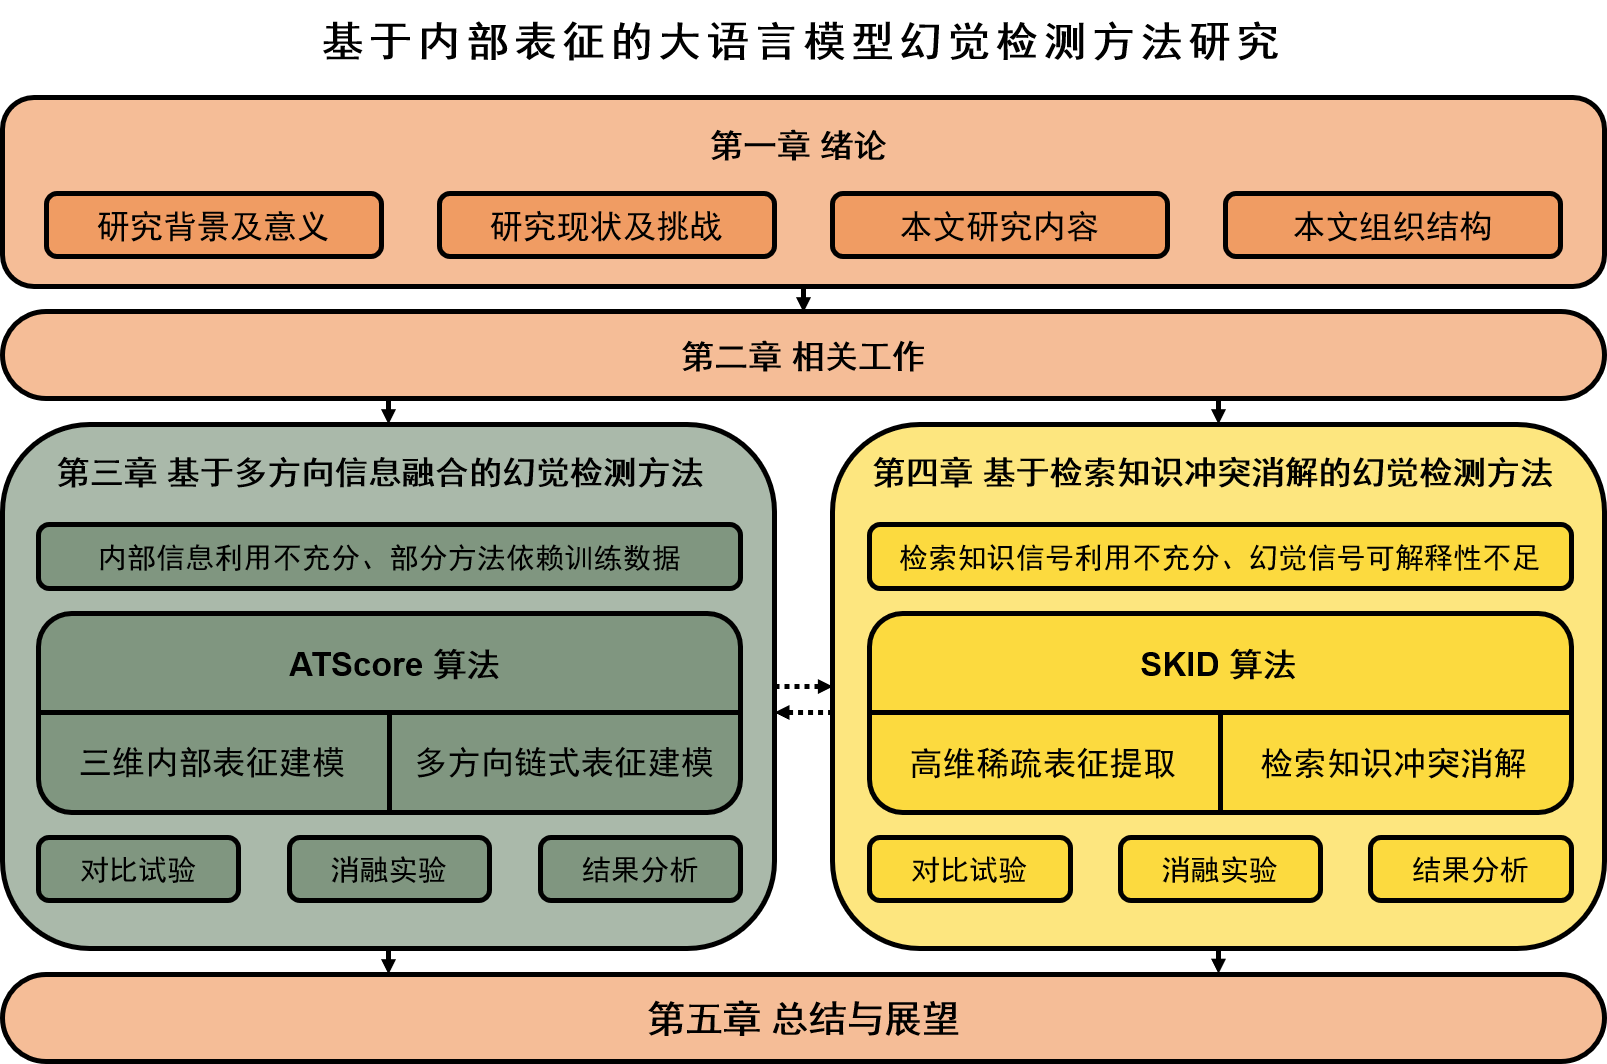
\includegraphics[width=\textwidth]{figures/content/总览.png}
    \caption{本文组织结构图}\label{fig:organization}
\end{figure}

% TODO：图片待改进
